%
% This is the LaTeX template file for lecture notes for EE 382C/EE 361C.
%
% To familiarize yourself with this template, the body contains
% some examples of its use.  Look them over.  Then you can
% run LaTeX on this file.  After you have LaTeXed this file then
% you can look over the result either by printing it out with
% dvips or using xdvi.
%
% This template is based on the template for Prof. Sinclair's CS 270.

\documentclass[twoside]{article}
\usepackage{graphicx}
\usepackage{algorithm}
\usepackage{algpseudocode}
\usepackage{graphics}
\usepackage{multicol}
\usepackage{amsmath} 
\setlength{\oddsidemargin}{0.25 in}
\setlength{\evensidemargin}{-0.25 in}
\setlength{\topmargin}{-0.6 in}
\setlength{\textwidth}{6.5 in}
\setlength{\textheight}{8.5 in}
\setlength{\headsep}{0.75 in}
\setlength{\parindent}{0 in}
\setlength{\parskip}{0.1 in}

%
% The following commands set up the lecnum (lecture number)
% counter and make various numbering schemes work relative
% to the lecture number.
%
\newcounter{lecnum}
\renewcommand{\thepage}{\thelecnum-\arabic{page}}
\renewcommand{\thesection}{\thelecnum.\arabic{section}}
\renewcommand{\theequation}{\thelecnum.\arabic{equation}}
\renewcommand{\thefigure}{\thelecnum.\arabic{figure}}
\renewcommand{\thetable}{\thelecnum.\arabic{table}}

%
% The following macro is used to generate the header.
%
\newcommand{\lecture}[4]{
   \pagestyle{myheadings}
   \thispagestyle{plain}
   \newpage
   \setcounter{lecnum}{#1}
   \setcounter{page}{1}
   \noindent
   \begin{center}
   \framebox{
      \vbox{\vspace{2mm}
    \hbox to 6.28in { {\bf EE 382C/361C: Multicore Computing
                        \hfill Fall 2016} }
       \vspace{4mm}
       \hbox to 6.28in { {\Large \hfill Lecture #1: #2  \hfill} }
       \vspace{2mm}
       \hbox to 6.28in { {\it Lecturer: #3 \hfill Scribe: #4} }
      \vspace{2mm}}
   }
   \end{center}
   \markboth{Lecture #1: #2}{Lecture #1: #2}
   %{\bf Disclaimer}: {\it These notes have not been subjected to the
   %usual scrutiny reserved for formal publications.  They may be distributed
   %outside this class only with the permission of the Instructor.}
   \vspace*{4mm}
}

%
% Convention for citations is authors' initials followed by the year.
% For example, to cite a paper by Leighton and Maggs you would type
% \cite{LM89}, and to cite a paper by Strassen you would type \cite{S69}.
% (To avoid bibliography problems, for now we redefine the \cite command.)
% Also commands that create a suitable format for the reference list.
\renewcommand{\cite}[1]{[#1]}
\def\beginrefs{\begin{list}%
        {[\arabic{equation}]}{\usecounter{equation}
         \setlength{\leftmargin}{2.0truecm}\setlength{\labelsep}{0.4truecm}%
         \setlength{\labelwidth}{1.6truecm}}}
\def\endrefs{\end{list}}
\def\bibentry#1{\item[\hbox{[#1]}]}

%Use this command for a figure; it puts a figure in wherever you want it.
%usage: \fig{NUMBER}{SPACE-IN-INCHES}{CAPTION}
\newcommand{\fig}[3]{
			\vspace{#2}
			\begin{center}
			Figure \thelecnum.#1:~#3
			\end{center}
	}
% Use these for theorems, lemmas, proofs, etc.
\newtheorem{theorem}{Theorem}[lecnum]
\newtheorem{lemma}[theorem]{Lemma}
\newtheorem{proposition}[theorem]{Proposition}
\newtheorem{claim}[theorem]{Claim}
\newtheorem{corollary}[theorem]{Corollary}
\newtheorem{definition}[theorem]{Definition}
\newenvironment{proof}{{\bf Proof:}}{\hfill\rule{2mm}{2mm}}

% **** IF YOU WANT TO DEFINE ADDITIONAL MACROS FOR YOURSELF, PUT THEM HERE:

\begin{document}
%FILL IN THE RIGHT INFO.
%\lecture{**LECTURE-NUMBER**}{**DATE**}{**LECTURER**}{**SCRIBE**}
\lecture{3}{September 1}{Vijay Garg}{Aditi Ranganath}
%\footnotetext{These notes are partially based on those of Nigel Mansell.}
% **** YOUR NOTES GO HERE:
% Some general latex examples and examples making use of the
% macros follow.  
%**** IN GENERAL, BE BRIEF. LONG SCRIBE NOTES, NO MATTER HOW WELL WRITTEN,
%**** ARE NEVER READ BY ANYBODY.
\section{Introduction}
In this lecture we will discuss various mutual exclusion protocols that work for {\em n} threads, where n is greater than 2. The scope of this lecture extends to the following algorithms : 

\begin{enumerate}
    \itemsep0em
    \item Proof of Peterson's algorithm (Review)
    \item Filter algorithm (Peterson-n algorithm)
    \item Tournament algorithm
    \item Bakery algorithm
\end{enumerate}



\section{Peterson's Algorithm (continued)}
So far we have developed an informal and a formal proof (Dijktra's proof) for Peterson's two-thread algorithm and discussed the concepts of $Deadlock\ Freedom$ and $Mutual\ Exclusion$ for the same.

\begin{table}[ht]
    \centering
    \begin{tabular}{l | l}
        Thread 0 ($P_0$):    & Thread 1 ($P_1$): \\
        \hline
        wantCS[0] $=$ true;                        &\ \ wantCS[1] $=$ true; \\
        turn $=$ 1;                                &\ \ turn $=$ 0; \\
        while\ (wantCS[1]\ \&\&\ (turn$==$1))\ ;\  &\ \ while\ (wantCS[0]\ \&\&\ (turn$==$0))\ ;\\
        $< critical\ section >$                    &\ \ \  $< critical\ section >$ \\
       wantCS[0] $=$ false;                        &\ \ \ wantCS[1] $=$ false; \\
        \hline
    \end{tabular}
\caption {Peterson's algorithm for two threads $P_0$ and $P_1$.}
\end{table}

In case of $Deadlock\ Freedom$, combining the conditions in which both $P_0$ and $P_1$ are waiting leads to contradiction, hence proving that the algorithm is starvation-free or deadlock-free. That is:
\begin{align*}
    (wantCS[1]\ \&\&\ (turn==1))\ \&\&\ (wantCS[0]\ \&\&\ (turn==0))
\end{align*}
On simplifying, we get \ (turn$==$1) \&\& (turn$==$0) \ which cannot be true.

In case of $Mutual\ Exclusion$, we used auxiliary variables $trying[0]$ and $trying[1]$ to prove by Dijktra's method that $P_1$ cannot falsify predicate $H[0]$ set by $P_0$ and vice versa, where, $H[0]$ is defined as:
\begin{align*}
    H[0] = wantCS[0]\ \&\&\ ( (turn==1) || ((turn==0)\&\&(trying[1])))
\end{align*}
On simplifying, we again get the contradiction case where\ (turn$==$1) \&\& (turn$==$0) \ which cannot be true. Thus, Peterson's algorithm for two threads is both $Deadlock\ Free$ and $Mutually\ Exclusive$ \cite{1}.



\section{Filter Algorithm: Peterson-n Algorithm}
We now try to extend Peterson's mutual exclusion protocol to work for $n(>2)$ threads. For this, we keep the algorithm to be symmetric and instead of the semantic $turn$, we use the variable $last$. We expect this to work well as it is easier to know which process wrote into the shared variable at the end.
Thus, for $P_i$ processes, where $i\in\{0,1,2,..,N-1\}$, we have

\begin{table}[ht]
    \centering
    \begin{tabular}{l}
       wantCS[i] = true;                                     
    \\ last = i;                                              
    \\ while(\ ($\exists$\ j:\ j$\neq$i:\ wantCS[j])\ \&\&\ (last$==$i)\ )\ ;    
    \\ $< critical\ section >$                                            
    \\ wantCS[i] = false;                                       
    \end{tabular}
\end{table} 

Now, lets examine if this is $Mutually\ Exclusive$ : Consider three processes $P_0$, $P_1$ and $P_2$. If $P_2$ was the last to write into the shared variable, only $P_2$ waits. Both $P_0$ and $P_1$ can now enter the critical section. This is not good as there is no $Mutual\ Exclusion$. If $n$ threads are at the gate at the same instance of time, only the last one is waiting while the remaining $(n-1)$ enter. In order to ensure only one thread enters the $critical\ section$, we have to repeat this process $(n-1)$ times. Thus, at each of the $(n-1)$ gates, we have one thread waiting which allows only one thread to enter the $critical\ section$ thereby ensuring $Mutual\ Exclusion$. With this, the algorithm looks as follows:

\begin{table}[ht]
    \centering
    \begin{tabular}{ l  l }
         int n;  \\
         int [n]gate; \\
         int [n]last init 0; &  $//\ last[0]\ will\ not\ be\ used$ \\
         for\ (int k$=$1\ ;\ k$<$n\ ;\ k$++$) \{\ & $//entry\ protocol$ \\
         \ \ \ \ gate[i]$=$k; & $//\ P_i\ is\ at\ gate\ k\ now$ \\
         \ \ \ \ last[k]$=$i; & $//\ P_i\ updates\ variable\ last\ for\ that\ gate$\\
         \ \ \ \ for\ (int j$=$0\ ;\ j$<$n\ ;\ j$++$) \{ & \\
         \ \ \ \ \ \ \ \ while(\ (j$\neq$i)\ \&\&\ (gate[j]$\geq$k)\ \&\&\ (last[k]$==$i)\ )\ ;&\\
         \ \ \ \ \} & $//inner\ for-loop$\\
         \} & $//outer\ for-loop$\\
         $<\ critical\ section\ >$ & \\
         gate[i]$=$0; & $//exit\ protocol$ \\
    \end{tabular}
\end{table} 

where, $i$ is the process index and $k$ is the gate index. Every process should go through $(n-1)$ gates to enter the $critical\ section$. Thus, Filter Algorithm can be visualized to be stacking of Peterson's algorithm on one another $(n-1)$ times with the following complexity:\\
Space complexity : $O(N)$ \\
Time complexity : $O(N^2)$ \\
On further analysis of the above algorithm, it can be shown that if process $P_i$ is pausing at any point, other processes $P_j$, $P_k$, etc. can enter $critical\ section$ overtaking $P_i$ arbitrary number of times.



\section{Tournament Algorithm}
Another simple technique to extend the use of a two-thread mutual exclusion algorithm for $n$ threads in using the Tournament Algorithm. In this case, each thread is progressing from the leaf to the root of the tree by participating in a two-thread mutual exclusion algorithm at every step. Thus, a thread has to pass through $log_2$(N) locks to enter the $critical\ section$. 

\begin{figure}[ht]
    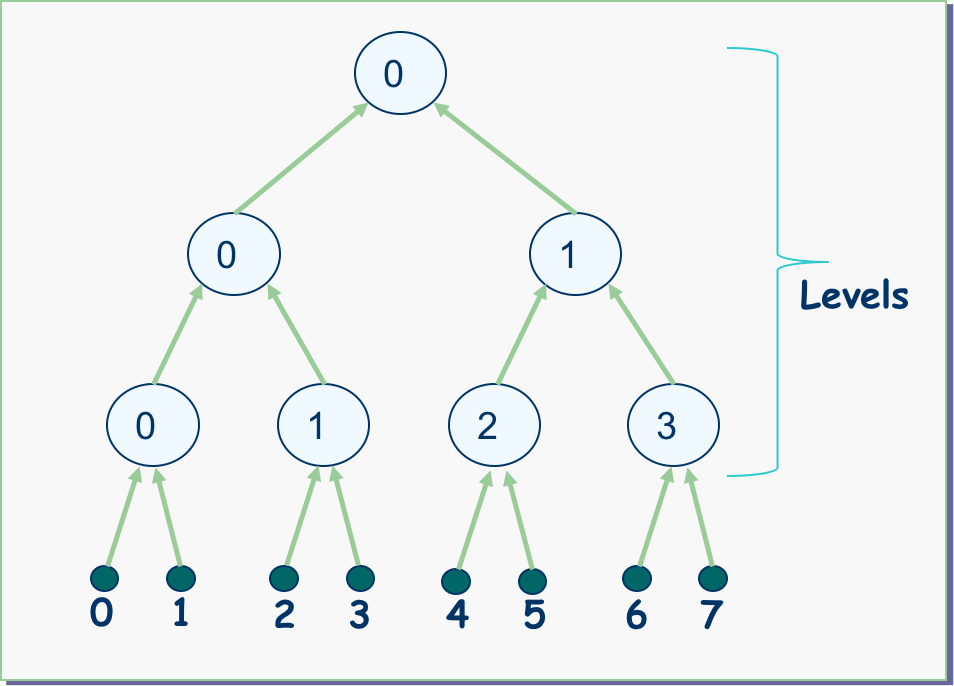
\includegraphics[scale=0.5]{Tournament_tree}
    \centering
    \caption{Tournament tree with multiple nodes and levels}
\end{figure}



\section{Variable read-write Atomicity}
A programming language can have three types of variables:
\begin{itemize}
    \itemsep0em
    \item SRSW : single-reader, single-writer variable
    \item MRSW : multi-reader, single-writer variable
    \item MRMW : multi-reader, multi-writer variable
\end{itemize}

Intuitively, in both SRSW and MRSW, the write order is deterministic. SRSW does not have any concurrency issues. MRSW also possesses sequential consistency but needs some checks for certain scenarios where concurrent reads can possibly return different values. However, in case of MRMW, the writes depend on the time stamps at which the request was made, and hence it requires more checks and locks. 

In $Filter\ algorithm$, we use a MRMW variable $last$ which requires some sort of atomicity and mutual exclusion for writes. Thus $Filter\ algorithm$ assumes mutual exclusion for the multi-writer variable.
This scenario can be avoided using the Lamport's Bakery Algorithm.



\section{Bakery Algorithm}
The algorithm was developed by Leslie Lamport with an analogy of a bakery with a numbering machine at its entrance so each customer is given a unique number. Numbers increase by one as customers enter the store. A global counter displays the number of the customer that is currently being served. All other customers must wait in a queue until the baker finishes serving the current customer and the next number is displayed. When the customer is done shopping and has disposed the number, the clerk increments the number, allowing the next customer to be served. That customer must draw another number from the numbering machine in order to shop again \cite{2}.
Extending this analogy, we have a scenario where every thread has a notion of its own number that can be written on only by itself but multiple threads can read from it. Thus, the algorithm uses a MRSW variable and eliminates the need for MRMW variable. The algorithm works as follows:

\begin{enumerate}
    \itemsep0em
    \item Every thread enters through a 'doorway' where it takes a number. This thread reads other threads' numbers to ensure it gets the biggest number.
    \item Ideally, only one thread should be at the doorway at a given time to get its number. However, it is possible that two threads enter the bakery at the same time and get the same number. To avoid concurrency issues, a unique ID is issued sequentially from 0 to $(n-1)$ to $n$ threads that enter simultaneously.
    \item Once a thread is inside the bakery, it waits till its number is the lowest in the bakery. The lowest thread enters the critical section.
    \item If multiple threads have the same number, the one with the lowest unique ID enters the critical section.
\end{enumerate}

\begin{table}[ht]
    \centering
    \begin{tabular}{l  l}
         boolean [ ]choosing; & $//init\ false$ \\
         int [ ]number; & $//init\ 0$ \\
         choosing[i]$=$true; & $//Step\ 1$ \\
         int t$=$max(number[0],.....,number[n-1]); & \\
         number[i]$=$t$+$1; & \\
         choosing[i]$=$false; & \\
         for(int j$=$0;\ j$<$n;\ j$++$) \{ & $//Step\ 2$ \\
         \ \ while(choosing[j])\ ; & $//avoid\ conflict$ \\
         \ \ while((number[j]$\neq$0)\&\&(number[j]$<$number[i])$||$(number[j]$==$number[i]\&\&(j$<$i))); & \\
         \} & $//end\ of\ for\ loop$ \\
         $ <\ critical\ section\ > $ & \\
         number[i]$=$0; & \\
    \end{tabular}
\end{table} 

\textbf{Proof}:\\
If $P_i$ is in critical section and $P_k$ (k$\neq$i) has already chosen its number, then, 
$(number[i], i)<(number[k], k)$ \\
Let $t$ be the time whrn $P_i$ checked choosing [k] and found it false. We have the following two cases:

\begin{figure}[ht]
    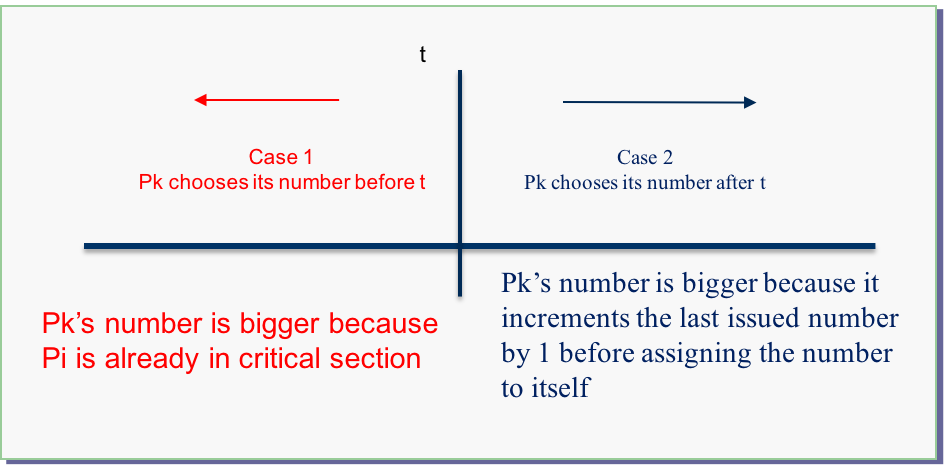
\includegraphics[scale=0.5]{Bakery_proof}
    \centering
    \caption{Two cases in Bakery algorithm}
\end{figure}

Thus, no matter when the number is chosen, the thread in the $critical\ section$ is the one with the smallest number. 



\section*{References}
\beginrefs
\bibentry{1}{\sc V.K.~Garg} Introduction to Multicore Computing
\bibentry{2} https://en.wikipedia.org/wiki/Lamport%27s_bakery_algorithm
\endrefs


\end{document}

